\section{Wegematrix}
\begin{frame}
	\frametitle{Wegematrix}
	\begin{definition}
    So wie Adjazenzmatrizen die Kantenrelation $E$ darstellen wollen wir jetzt die Erreichbarkeitsrelation $E^*$ darstellen.\\
		$E^* := \bigcup \limits^{\infty}_{i=0} E^i $. \\
    Wir nennen die Matrixdarstellung von $E^*$ die \emph{Wegematrix} $W$.
   \begin{displaymath}
     W_{ij} :=
      \begin{cases}
        1, & \text{falls es in G einen Pfad von i nach j gibt} \\
        0, & \text{falls es in G keinen Pfad von i nach j gibt}
      \end{cases}
    \end{displaymath}
	\end{definition}
\end{frame}

\begin{frame}
	\frametitle {Beispiel}
	\begin{columns}
		\column{.5\textwidth}
		\begin{center}
		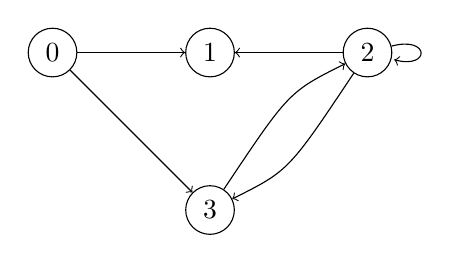
\begin{tikzpicture}
		  \tikzstyle{every node}=[draw,shape=circle];
			\path[fill] (0,0)  node[circle] (0) {0};
			\path[fill] (2,0)  node[circle] (1) {1};
			\path[fill] (4,0)  node[circle] (2) {2};
			\path[fill] (2,-2) node[circle] (3) {3};

			\path[->,draw] (0) -- (1);
			\path[->,draw] (2) -- (1);
			\path[->,draw] (2) edge [loop right] ();
			\path[->,draw] (3) .. controls (3,-0.5) ..  (2);
			\path[->,draw] (2) .. controls (3,-1.5) ..  (3);
			\path[->,draw] (0) -- (3);
		\end{tikzpicture}
		\end{center}
    \column{.5\textwidth}
        $A = $
				$\left(
						\begin{matrix}
							0 & 1 & 0 & 1 \\
							0 & 0 & 0 & 0 \\
							0 & 1 & 1 & 1 \\
							0 & 0 & 1 & 0
						\end{matrix}
				\right)$
	\end{columns}
	\begin{block}{Fragen}
		\begin{itemize}
			\item Wie sieht die Wegematrix zum oben gezeigten Graph aus?
			\visible<2->{\item Wie sieht die Wegematrix für eine vollständig mit 1en gefüllte Matrix aus?}
			\visible<3->{\item Wann gilt allgemein $W=A$? Wann gilt $E^1=A$?}
		\end{itemize}
	\end{block}
\end{frame}

\subsection{Algorithmen}

\begin{frame}[fragile]
	\frametitle{Algorithmus zur Wegematrix}
  \begin{lstlisting}[language = Java,mathescape,morekeywords={set}]
    // Eingabe: A: Adjazenzmatrix
    // Ausgabe: W Wegematrix

    W = 0 // Nullmatrix
    for i = 0 to n - 1 do
      M = Id // Einheitsmatrix
      for j = 1 to i do
        M = M $\cdot$ A
      od
      W = W + M
    od
    W = sgn$(W)$
  \end{lstlisting}
\end{frame}

\begin{frame}[fragile]
	\frametitle{Algorithmus zur Wegematrix}
  \begin{lstlisting}[language = Java,mathescape,morekeywords={set}]
    // Eingabe: A: Adjazenzmatrix
    // Ausgabe: W Wegematrix

    W = 0 // Nullmatrix
    M = Id // Einheitsmatrix
    for i = 0 to n - 1 do
      W = W + M
      M = M $\cdot$ A
    od
    W = sgn$(W)$
  \end{lstlisting}
\end{frame}

\begin{frame}
	\frametitle{Aufwand}
	\begin{block}{Zählweise}
		Beim Vergleich verschiedener Algorithmen in Bezug auf den Aufwand, sucht man nach einem Maß für die Anzahl der Rechenoperationen für eine Aufgabe der Größe $n$.
	\end{block}
	\begin{block}{Beispiel} \pause
		Summe aller Zahlen von $1$ bis $n$: \\
			$\sum^n_{i=0} i = $\pause$n*(n+1)/2$
	\end{block}
\end{frame}

\begin{frame}
	\begin{block}{Aufwandsvergleich}
		Wenn man in einem bestimmten Zeitraum mit dem $n^5$ Algorithmus gerade noch die Problemgröße $n=1000$ schafft:
	  \begin{itemize}
		  \item Wie große Probleminstanzen schafft man mit dem $n^4$ Algorithmus? \pause
		  \item ... oder mit dem $log_2(n) \cdot n^3$ Algorithmus?
	  \end{itemize}
	\end{block}
\end{frame}

\section{Warshall-Algorithmus}
\subsection*{}
\begin{frame}
	\frametitle{Reflexive Transitive Hülle nach Warshall}
	Wir definieren eine Relation $\sigma^{(k)}$ über $V=\{0,\dots,n-1\}$ mit:
		$\sigma^{(k)} = \{(i,j) \in V \times V |$
    $ \exists p = (i, v_1, \cdots, v_n, j) \in V^+$ mit:\\
    \hfill alle inneren Knoten $v_i \in \{0, \cdots, k\}\}$

	\begin{columns}
	\column{.2\textwidth}
		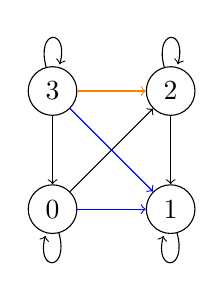
\begin{tikzpicture}
		  \tikzstyle{every node}=[draw,shape=circle];
			\path[fill] (0,0)  node[circle] (0) {0};
			\path[fill] (1.5,0)  node[circle] (1) {1};
			\path[fill] (1.5,1.5)  node[circle] (2) {2};
			\path[fill] (0,1.5)  node[circle] (3) {3};

			\path[->,draw] (0) edge [loop below] ();
			\path[->,draw] (1) edge [loop below] ();
			\path[->,draw] (2) edge [loop above] ();
			\path[->,draw] (3) edge [loop above] ();
			\path[->,draw] (3) -- (0);
			\path[->,draw] (0) -- (2);
			\path[->,draw] (2) -- (1);
			\visible<2->{\path[->,draw,orange] (3) -- (2);}
			\visible<6->{\path[->,draw,blue] (3) -- (1);}
			\visible<6->{\path[->,draw,blue] (0) -- (1);}
		\end{tikzpicture}
	\column{.4\textwidth}
		\[
		{\color{orange} W_{(0)}}=\
		\alt<2->{
			\left(
			\begin{matrix}
			1 & 0 & 1 & 0\\
			0 & 1 & 0 & 0\\
			0 & 1 & 1 & 0\\
			1 & 0 & {\color{orange}1} & 1
			\end{matrix}
			\right)
		}{
			\left(
			\begin{matrix}
			1 & 0 & 1 & 0\\
			0 & 1 & 0 & 0\\
			0 & 1 & 1 & 0\\
			1 & 0 & 0 & 1
			\end{matrix}
			\right)
		}
		\]
		\[
		\visible<5->{
			{ \color{blue} W_{(2)}}=\
		}
		\alt<-5>{
			\visible<5->{
				\left(
				\begin{matrix}
				1 & 0 & 1 & 0\\
				0 & 1 & 0 & 0\\
				0 & 1 & 1 & 0\\
				1 & 0 & {\color{orange}1} & 1
				\end{matrix}
				\right)
			}
		}
		{
			\left(
			\begin{matrix}
			1 & {\color{blue} 1} & 1 & 0\\
			0 & 1 & 0 & 0\\
			0 & 1 & 1 & 0\\
			1 & {\color{blue} 1} & {\color{orange}1} & 1
			\end{matrix}
			\right)
		}
		\]
	\column{.4\textwidth}
		\[
		\visible<3->{
			{ \color{green} W_{(1)}}=\
		}
		\alt<-3>{
			\visible<3->{
				\left(
				\begin{matrix}
				1 & 0 & 1 & 0\\
				0 & 1 & 0 & 0\\
				0 & 1 & 1 & 0\\
				1 & 0 & {\color{orange}1} & 1
				\end{matrix}
				\right)
			}
		}
		{
			\left(
			\begin{matrix}
			1 & 0 & 1 & 0\\
			0 & 1 & 0 & 0\\
			0 & 1 & 1 & 0\\
			1 & 0 & {\color{orange}1} & 1
			\end{matrix}
			\right)
		}
		\]
		\[
		\visible<7->{
			{ \color{red} W_{(3)}}=\
		}
		\alt<-7>{
			\visible<7->{
				\left(
				\begin{matrix}
				1 & {\color{blue} 1} & 1 & 0\\
				0 & 1 & 0 & 0\\
				0 & 1 & 1 & 0\\
				1 & {\color{blue} 1} & {\color{orange}1} & 1
				\end{matrix}
				\right)
			}
		}
		{
			\left(
			\begin{matrix}
			1 & {\color{blue} 1} & 1 & 0\\
			0 & 1 & 0 & 0\\
			0 & 1 & 1 & 0\\
			1 & {\color{blue} 1} & {\color{orange}1} & 1
			\end{matrix}
			\right)
		}
		\]
	\end{columns}
\end{frame}

\begin{frame}[fragile]
	\frametitle{Der Warshall-Algorithmus}
  \begin{lstlisting}[language = Java,mathescape,morekeywords={set}]
    \\ Eingabe: A Adjanzenzmatrix
    \\ Ausgabe: W Wegematrix
    $W$ := $A$
    for i=0 to n-1 do
      $W[i,i]$ = $1$

    for k=0 to n-1 do
      for i=0 to n-1 do
        for j=0 to n-1 do
          $W[i,j] = max\{W[i,j], min\{W[i,k], W[k, j]\}\}$
  \end{lstlisting}
\end{frame}

\subsection{Aufgaben}
\begin{frame}[fragile]
  \frametitle{Aufgaben}
      Berechnet mit dem Algorithmus von Warshall die Wegematrix.\\
      Gebt nach jedem Durchlauf der äußersten Schleife $W_k$ an.
      \begin{center}
        \begin{tikzpicture}[->,>=stealth,baseline=-5mm]
          \matrix[matrix of math nodes,nodes={draw,circle,minimum size=5mm,inner sep=2pt},row sep=10mm,column sep=10mm]
          {
            |(0)| 0 & |(1)| 1 & |(2)| 2 \\
            & |(3)| 3 & \\
          };
          \draw  (0) -- (1);
          \draw  (2) -- (1);
          \draw  (1) to [bend left] (3);
          \draw  (3) to [bend right] (2);
          \path (1) edge [loop above] ();
        \end{tikzpicture}
      \end{center}
\end{frame}

\begin{frame}
	\frametitle{Klausuraufgabe WS 2010/2011 - Nr.2}
	Für $n\in \mathbb{N}_0, n \geq 2$ sei ein Graph $U_n=(\mathbb{G}_{2n},E_n)$ definiert mit Kantenmenge $E_n=\{\{x,y\}|\text{ggT}(x+y,2n)=1\}$.\\
	\vspace{.2cm}
	\begin{exampleblock}{Zur Erinnerung:}
		\begin{itemize}
			\item $\forall m\in \mathbb{N}_0: \mathbb{G}_m=\{i|0\leq i<m\}$
			\item $\text{ggT}(x,y)$ ist der kleinste gemeinsame Teiler von $x$ und $y$
		\end{itemize}
	\end{exampleblock}
	\begin{description}
		\item[a)] Zeichnen Sie die Graphen $U_3$, $U_4$ und $U_5$.
		\item[b)] Geben sie für $U_4$ und $U_5$ jeweils einen Weg an, bei dem der Anfangsknoten gleich dem Endknoten ist und jeder andere Knoten des Graphen genau einmal in dem Weg vorkommt.
		\item[c)] Geben Sie die Adjazenzmatrix für $U_4$ an.
	\end{description}
\end{frame}
